\scanpage{51}
- \mspage{4} -

sion d'une variété abélienne par un tore. Alors, pour que $G$ \deleted{es} ait \inserted{``}bonne réduction\inserted{''} sur $S$, \inserted{\figure{\begin{tikzpicture}\node[draw,ellipse] (a) {de car. rés. $p>0$};\draw (a.south west)..controls(-2,-.7)..(-2.3,-1.2);\end{tikzpicture}}} il faut et il suffit que le groupe p-divisible $\underset{\sim}{G}$ se prolonge en un S-groupe p-divisible.

\margin{\figure{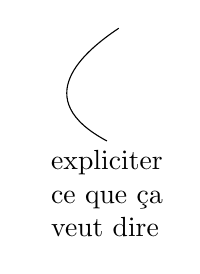
\begin{tikzpicture}\node[align=left] (a) {expliciter\\ce que ça\\veut dire};\draw (a.north)..controls(-1,1.2)and(-.3,1.8)..(.15,2.1);\end{tikzpicture}}}

\mspage{50}
